\documentclass[journal,twoside,web]{ieeecolor}
\usepackage{cite}
\usepackage{generic}
\usepackage{bm}
\usepackage{pifont}
\usepackage{multirow}
\usepackage{booktabs}
\usepackage{array}
\usepackage{threeparttable}
\usepackage{amsmath,amssymb,amsfonts}
\usepackage{graphicx}
\usepackage{textcomp}
\usepackage{mathtools} 
\usepackage{float}

\def\BibTeX{{\rm B\kern-.05em{\sc i\kern-.025em b}\kern-.08em
    T\kern-.1667em\lower.7ex\hbox{E}\kern-.125emX}}
\markboth{\journalname, VOL. XX, NO. XX, XXXX 2023}
{Wang \MakeLowercase{\textit{et al.}}: Graph convolutional network for predicting miRNA-disease associations}

\begin{document}
\title{Meta-path semantic and global-local representation learning enhanced graph convolutional model for disease-related miRNA prediction}
\author{Ping Xuan, Xiuju Wang, Hui Cui, Xiangfeng Meng, Toshiya Nakaguchi and Tiangang Zhang\,$^{*}$
\thanks{The work was supported by the Natural Science Foundation of China (61972135,62172143); STU Scientific Research Initiation Grant (NTF22032); China Postdoctoral Science Foundation (2019M650069, 2020M670939); Heilongjiang Postdoctoral Scientific Research Staring Foundation (BHLQ18104); and Foundation of Graduate Innovative Research (YJSCX2022-235HLJU).}
\thanks{Ping Xuan is with the Department of Computer Science, School of Engineering, Shantou University, Shantou, 515063, China.}
\thanks{Xiuju Wang is with the School of Computer Science and Technology, Heilongjiang University, Harbin 150080, China.}
\thanks{Hui Cui is with the Department of Computer Science and Information Technology, La Trobe University, Melbourne, 3083, Australia.}
\thanks{Xiangfeng Meng is with the School of Computer Science and Technology, Heilongjiang University, Harbin 150080, China.}\thanks{Toshiya Nakaguchi is with the Center for Frontier Medical Engineering, Chiba University, Chiba 2638522, Japan.}
\thanks{Tiangang Zhang is the corresponding author and he is with the School of Mathematical Science, Heilongjiang University, Harbin, 150080, China (e-mail: zhang@hlju.edu.cn).}
}

\maketitle

\begin{abstract}
Dysregulation of miRNAs is closely related to the progression of various diseases, so identifying disease-related miRNAs is crucial. Most recently proposed methods are based on graph reasoning, while they overlook the topological structure composed of the higher-order neighbor nodes. We proposed a prediction method, MDAP, to learn semantic features of miRNA and disease nodes based on various meta-paths, as well as node features from the entire heterogeneous network perspective, and node pair attributes. Firstly, for both the miRNA and disease nodes, node category-wise meta-paths were constructed to integrate the similarity and association connection relationships. Each target node has its specific neighbor nodes for each meta-path, and the neighbors of longer meta-paths constitute its higher-order neighbor topological structure. Secondly, we constructed a meta-path specific graph convolutional network module to integrate the features of higher-order neighbors and their topology, and then learned the local semantic representations of nodes. Thirdly, for the entire miRNA-disease heterogeneous network, a module based on graph convolutional autoencoder was built to learn the global network-view feature representations of nodes. We also designed semantic-level and representation-level attentions to obtain informative semantic features and node representations. Finally, the strategy based on the parallel convolutional-deconvolutional neural networks was designed to enhance the local feature learning for a pair of miRNA and disease nodes. The experiment results showed that MDAP outperformed other state-of-the-art methods, and the ablation experiments demonstrated the effectiveness of MDAP’s major innovations. MDAP’s ability in discovering potential disease-related miRNAs was further analyzed by the case studies over three diseases.
\end{abstract}

\begin{IEEEkeywords}
semantic feature learning based on various meta-paths, higher-order neighbor topological structure integration, pairwise local feature learning, disease-related miRNA prediction, deep learning.
\end{IEEEkeywords}

\section{Introduction}
\label{sec:introduction}
\IEEEPARstart{M}{icroRNAs} (miRNAs) are small non-coding RNAs with a length of 22–24 nucleotides \cite{Luca2018Regulation,DBLP:journals/bib/ChenHWYSW19}. Abnormalities in miRNAs have been associated with the development of various diseases \cite{2019MicroRNAs,ijms21010132}. For this reason, identifying disease-associated miRNAs can help explore the pathogenesis of diseases and facilitate their diagnosis and treatment. Calculating the likelihood of predicting miRNAs associated with diseases can assist in the selection of candidate miRNAs for each disease, reducing the cost and time required for biological experiments.

The three major categories of existing miRNA-disease association prediction methods are as follows. The biological premise underlying the first group of methods is that miRNAs are more likely to be associated with comparable diseases when their functions are similar \cite{2019Adaptive}. Thus, the functional similarity of miRNAs is determined using the diseases related to the two miRNAs \cite{2010Inferring}. Chen {\it et al.} \cite{2012RWRMDA} and Xuan {\it et al.} \cite{2015Prediction} performed random walk (RW) on miRNA similarity networks to infer the relevance of miRNAs to diseases. Information regarding the k most similar neighbor nodes of a miRNA was also utilized \cite{2013Prediction}. However, the aforementioned strategies are only appropriate for diseases that have known miRNAs associated with them and not for other diseases.

The strategies in the secondary category add extra diseases information to establish miRNA-disease heterogeneous networks to incorporate miRNA-disease association, miRNA similarity and disease similarity. In order to infer disease-associated candidate miRNAs, Chen {\it et al.} presented a ranking calculation technique based on k-nearest neighbors \cite{2017RKNNMDA}, and You {\it et al.} proposed a depth-first search technique \cite{2017PBMDA}. The miRNA-disease association score can also be obtained using random walk \cite{2021A, 2016Inferring,2017A , 2018Global}, regularized least squares \cite{2015Semi}, and miRNA-disease network projection \cite{2016Network, Chen2018BNPMDA}. Wang {\it et al.} introduced miRNA sequence information into their model and used a logic tree classifier for miRNA-disease association prediction \cite{2019LMTRDA}. Certain matrix decomposition-based techniques are also available \cite{20, 21, Ping2018Inferring, 2020NCMCMDA, 2018MDHGI}. However, these techniques use shallow prediction models that fail to adequately illuminate the deeper and more intricate connections between miRNAs and diseases.

The third category uses deep learning techniques to combine data on miRNAs and diseases to more precisely identify potential miRNA candidates linked to diseases. Convolutional neural network (CNN) based prediction models were proposed by Peng {\it et al.} \cite{Jiajie2019A} and Xuan {\it et al.} \cite{Ping2018Dual}. Network-based semi-supervised model of label propagation algorithms \cite{27} was developed to predict disease-associated candidate miRNAs. In addition, graph convolutional neural networks (GCN) \cite{2020FCGCNMDA, 2020Heterogeneous, 2020Neural}, generative adversarial networks \cite{0Integration}, autoencoders \cite{0AEMDA,33} and deep belief networks \cite{34} have been used to model miRNA-disease association candidate prediction. These models, which are based on deep learning, are more accurate predictors because they learn the intricate connections between miRNAs and diseases. Previous approaches have rarely focused on learning meta-path semantic information specific to different classes of nodes or capturing higher-order structures in heterogeneous networks.

We suggest a novel prediction method in this study called MDAP for learning meta-path semantics of multiple types of nodes and higher-order structures in a miRNA-disease heterogeneous network. The method leverages topological information of the entire network and diverse node-pair attribute information. The following is a summary of our model's contributions.

\begin{itemize}
   \item A heterogeneous network is firstly constructed and it consists of the miRNA and disease nodes, and the similarity connections and the association ones among them. There are long-distance dependencies among the nodes in the miRNA-disease network. Thus, we build multiple meta-paths to form the topological structures composed of high-order neighbors and learn the dependencies among these neighbors.
	\item The heterogenous network contains the miRNA nodes and the disease ones, and each type of nodes has their own meta-paths. Moreover, each meta-path has its specific semantic information and the topological structure formed by its neighbors. A meta-path-sensitive learning module is constructed based on graph convolutional networks, and it may learn the semantic features of each miRNA (disease) node for each meta-path. Since the multiple meta-paths of the miRNA (disease) nodes have different contributions to the semantic feature learning, the semantic-level attention is designed to discriminate their contributions.
	\item A module based on graph convolutional autoencoder is built to learn the network-view representations of the miRNA and disease nodes from the entire heterogeneous network perspective. Furthermore, the attention at the representation level is proposed to adaptively fuse the semantic representations and the network-view representations of the miRNA (disease) nodes.
	\item A module including both convolution networks and the deconvolution networks is designed to enhance the local feature learning for a pair of miRNA-disease nodes. The original feature map is stretched which make the module focus on learning the more local features. A comprehensive comparison with several recent prediction methods and the case studies over 3 diseases indicate our method's superior performance and its ability in retrieving the potential disease-related miRNAs.
\end{itemize}

\section{Materials and methods}
We proposed an association prediction model, MDAP, to predict potential miRNAs linked to a certain disease (Figure \ref{fig:01}). First, we learned semantic information about the meta-paths specific to miRNA- and disease-type nodes, as well as the higher-order structure of the heterogeneous network based on meta-path-specific graph convolution (GCN) (Figure \ref{fig:01}(a)). Then, we build a graph convolutional autoencoder (GCA) module to deeply integrate topological and node attributes in miRNA-disease heterogeneous networks (Figure \ref{fig:01}(b)). A node representation-level attention mechanism was designed to self-adapt to fuse meta-path semantic representations and network-view representations (Figure \ref{fig:01}(c)). In addition, we designed a parallel convolution and deconvolution network to encode the attributes of a pair of miRNA and disease nodes (Figure \ref{fig:01}(d)). 

%figure1 图注
\begin{figure*}
	\centering
	% requires \usepackage{graphicx}
	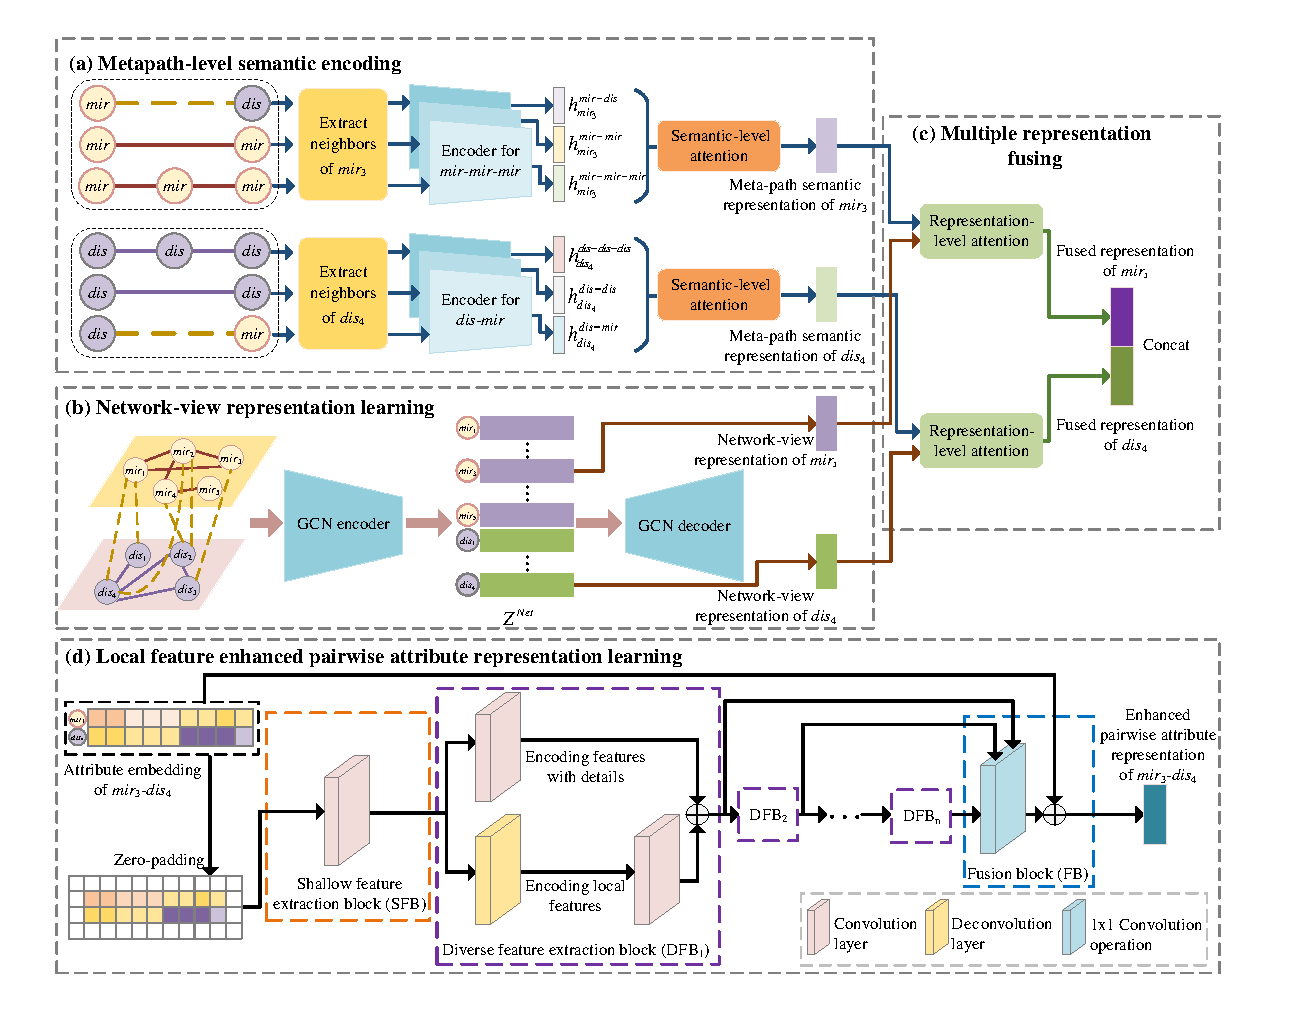
\includegraphics[width=6.9in]{fig/fig1.pdf}\\
	\caption{Framework of the proposed MDAP model. {\textbf{(a)} learn meta-path semantic representation of each miRNA (disease) node. \textbf{(b)} learn the network-view representations of nodes from the entire heterogeneous network perspective. \textbf{(c)} fuse multiple representations of nodes. \textbf{(d)} learn the local feature enhanced pairwise attribute representation.}}
    \label{fig:01}
	\vspace{-0.4cm}
\end{figure*}

\subsection{Dataset}

The Human MicroRNA Disease Database contains 7908 miRNA-disease correlations \cite{35}, and these associations cover 793 miRNAs and 341 diseases. We created directed acyclic graphs (DAGs) using the terminology for diseases from the American Library of Medicine \cite{0Meshable}. Based on their DAGs, the semantic similarity between the two diseases was determined \cite{2010Inferring}.

\subsection{Double-layer heterogeneous network and matrix}

A miRNA-disease double-layer heterogeneous network $G{\rm{ = }}\left( {V,E,W} \right)$ was created. The set of nodes $V = \left\{ {{V^{mir}} \cup {V^{dis}}} \right\}$, where ${V^{mir}}$ denotes ${N_m}$ miRNA nodes $\left\{ {mi{r_1},mi{r_2},...,mi{r_{{N_m}}}} \right\}$ and ${V^{dis}}$ denotes ${N_d}$ disease nodes $\left\{ {di{s_1},di{s_2},...,di{s_{{N_d}}}} \right\}$.
Edge ${e_{ij}} \in E$ with weight ${w_{ij}} \in W$ links a pair of nodes, ${v_i},{v_j} \in V$. There are two kinds of connections between nodes in $G$. One is the intra-layer connection between nodes of the same type, such as miRNA-miRNA similarity connection and disease-disease similarity connection. The other type is the inter-layer connection, including miRNA-disease association connection. We define $W = \left( {{A^{sim}},{B^{mir - dis}}} \right)$, where ${A^{sim}}$ is the intra-layer relationship matrix and ${B^{mir - dis}}$ is the inter-layer relationship matrix.

${A^{sim}}$ includes miRNA similarity and disease similarity matrices, defined as
\begin{equation}
{A^{sim}} = \left\{ {\begin{array}{*{20}{c}}
{{A^{mir}} \in {R^{{N_m} \times {N_m}}},{\rm{ }}if{\ \rm{  }}{\rm{  }}{\rm{  }}{v_i},{v_j} \in {V^{mir}}}\\
{{A^{dis}} \in {R^{{N_d} \times {N_d}}},{\rm{ }}if{\ \rm{  }}{\rm{  }}{\rm{  }}{v_i},{v_j} \in {V^{dis}}}\\
\end{array}} \right.,
\end{equation}
${A^{mir}}$ records similarities between ${N_m}$ miRNAs. The more similar the function of two miRNAs, the more likely they are to be associated with similar diseases. Based on this biological premise and influenced by the strategy of Wang {\it et al.} \cite{2010Inferring}, similarity $A_{ij}^{mir}$ between $mi{r_i}$ and $mi{r_j}$ is calculated using their association with the two groups of diseases. The DAG of a disease usually consists of the disease and its related terms and their associations \cite{2010Inferring}. Using the Wang {\it et al.} technique \cite{2010Inferring}, the semantic similarity $A_{ij}^{dis}$ between two diseases $di{s_i}$ and $di{s_j}$ is determined based on their DAGs. The higher the value of $A_{ij}^{mir}\left( {A_{ij}^{dis}} \right)$, the greater the similarity between $mi{r_i}\left( {di{s_i}} \right)$ and $mi{r_j}\left( {di{s_j}} \right)$.

${B^{mir - dis}}$ reflects the association between miRNAs and diseases,
\begin{equation}
B^{mir - dis}\in {R^{{N_m} \times {N_d}}},{\rm{ }}if{\ \rm{  }}{\rm{  }}{\rm{  }}{v_i} \in {V^{mir}},{\rm{ }}{v_j} \in {V^{dis}},
\end{equation}
each row of ${B^{mir - dis}}$ stands in for one miRNA and each column for one disease. In case $mi{r_i}$ and $di{s_j}$ are related, then $B_{ij}^{mir - dis} = 1$; otherwise, $B_{ij}^{mir - dis} = 0$.

Given the similarity matrix ${A^{mir}}$, ${A^{dis}}$ and association matrix ${B^{mir - dis}}$, the weight matrix of all edges in $G$ is
\begin{equation}
W = \left[ {\begin{array}{*{20}{c}}
{{A^{mir}}}&{{B^{mir - dis}}}\\
{{{\left( {{B^{mir - dis}}} \right)}^T}}&{{A^{dis}}}
\end{array}} \right] \in {R^{{N_v} \times {N_v}}},
\end{equation}
 where ${\left( {{B^{mir - dis}}} \right)^T}$ is the transpose matrix for ${B^{mir - dis}}$ and ${N_v} = {N_m} + {N_d}$. All nodes in $G$ are connected by edges to form the adjacency matrix $C$, $C = W$. For miRNA or disease nodes, the similarities and associations between them can be considered attributes of the nodes. Therefore, $W$ is considered the attribute matrix of nodes in $G$ and is denoted as $X$.
\begin{figure}[!t]
	\centering
	%\usepackage{float}
	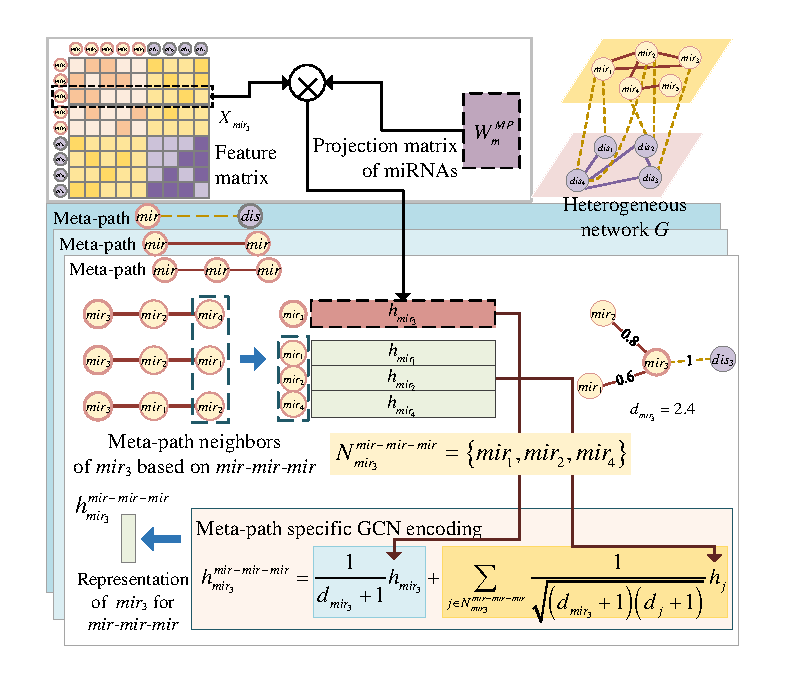
\includegraphics[width=3.5in]{fig/fig-2.pdf}\\
	\caption{ Illustration of meta-path specific GCN encoding for a miRNA node.}
	\label{fig:02}
	\vspace{-0.4cm}
\end{figure}

\subsection{Learning of semantic information based on various meta-paths}

A meta-path is defined as a path, such as ${D_1}\xrightarrow{{{r_1}}}{D_2}\xrightarrow{{{r_2}}}\cdot  \cdot  \cdot \xrightarrow{{{r_l}}}{D_{l + 1}}$ (abbreviated as ${D_1}{D_2} \cdot  \cdot  \cdot {D_{l + 1}}$ ), which describes the composite relationship between nodes ${D_1}$ and ${D_{l + 1}}$ \cite{37}. An instance of a meta-path is defined as a sequence of nodes that follow a defined pattern \cite{37}. For example, $mir\xrightarrow{{{r_1}}}mir\xrightarrow{{{r_2}}}dis$ denotes a meta-path of length two, ${r_1}$ denotes miRNA similarity, and ${r_2}$ denotes the miRNA-disease association. $mi{r_1} \to mi{r_3} \to di{s_9}$ is an instance of this meta-path, and $di{s_9}$ is the neighbor of $mi{r_1}$ based on this meta-path. Since different meta-paths contain various semantics, we built a meta-path-guided encoder to learn semantic information (Figure \ref{fig:02}).

Because the semantic coding process of miRNAs is similar to that of diseases, we used miRNA as the target node to explain this process. The feature vector of $mi{r_i}$ is called ${X_i} \in X$. First, we projected ${X_i}$ using the mapping matrix $W_m^{MP}$ of miRNA node types to form the projected feature vector ${h_i}$,
\begin{equation}
{h_i} = \mu \left( {W_m^{MP} \cdot {X_i} + b_m^{MP}} \right),
\end{equation}
where $\mu $ is the activation function $tanh$ and $b_m^{MP}$ denotes a bias vector. The type-specific mapping matrix for disease nodes is $W_d^{MP}$.

Given a meta-path ${q_m}$, $N_i^{{q_m}}$ is the set of neighboring nodes of $mi{r_i}$ corresponding to the meta-path. The topology and node attributes in ${q_m}$ are deeply fused to obtain the semantic feature $h_i^{{q_n}}$ of $mi{r_i}$ by meta-path specific GCN \cite{37}:
\begin{equation}
h_i^{{q_m}} = \frac{1}{{{d_i} + 1}}{h_i} + \sum\limits_{j \in N_i^{{q_{_m}}}} {\frac{1}{{\sqrt {\left( {{d_i} + 1} \right)\left( {{d_j} + 1} \right)} }}{h_j}},
\end{equation}
where ${h_i}$ and ${h_j}$ are the projected feature vectors of $mi{r_i}$ and its neighboring nodes, while ${d_i}$ and ${d_j}$ are degrees of the nodes.

Given a meta-path set ${Q_{mir}} = \left\{ {{q_1},{q_2},...,{q_{{N_p}}}} \right\}$, the ${N_p}$ semantic features $\left\{ {h_i^{{q_1}},...,h_i^{{q_{{N_p}}}}} \right\}$ of the target node $mi{r_i}$ are generated by meta-path specific GCN encoder. Because the semantic features implied by $h_i^{{q_1}},...,h_i^{{q_{{N_p}}}}$ contribute equally to the semantic representation learning of the meta-path of $mi{r_i}$, we design a semantic-level attention mechanism. The attention weight of the semantics implied by ${q_m}$ is ${\alpha _{i,{q_m}}}$,

\begin{equation}
{\alpha _{i,{q_m}}} = \frac{{\exp \left( {\rho \left( {{{\left( {u_i^{{q_m}}} \right)}^T}h_i^{{q_m}}} \right)} \right)}}{{\sum\nolimits_{s = 1}^{{N_p}} {\exp \left( {\rho \left( {{{\left( {u_i^{{q_s}}} \right)}^T}h_i^{{q_s}}} \right)} \right)} }},
\end{equation}
where $u_i^{{q_m}}$ denotes the trainable attention vector, $\exp $ is the exponential function, and $\rho $ is the activation function $LeakyReLU$.

The meta-path semantics representation of $mi{r_i}$ enhanced by attention, ${Z^{MP}}\left( i \right)$, is given as follows.
\begin{equation}
{Z^{MP}}\left( i \right) = \sum\limits_{s = 1}^{{N_p}} {\left( {{\alpha _{i,{q_s}}} \cdot h_i^{{q_s}} + h_i^{{q_s}}} \right)},
\end{equation} 
The meta-path semantic representations form matrix ${Z^{MP}}$. The meta-path semantic representation of disease node $di{s_j}$ is ${Z^{MP}}\left( {{N_m} + j} \right)$.

%2.4
\subsection{Learning of miRNA-disease heterogeneous network information}

The heterogeneous network $G$ contains diverse connections and various linkages between all miRNA and disease nodes, including similarity and association connections. There are contextual links between these connections. To fully capture their contextual connections, we built a module based on GCA to learn the information at the entire heterogeneous network view.

\textbf{GCN encoder.} ${C_{ii}}$ denotes the similarity between nodes ${v_i}$ and ${v_i}$. Therefore, the values on the diagonal of the adjacency matrix $C$ are all 1, indicating a connection between the node and itself. We fed $C$ and $X$ into GCN encoder. The $\varphi $th GCN encoding layer's output can be expressed as
\begin{equation}
{\left( {Z_{^{enc}}^{Net}} \right)^\varphi } = \theta \left( {{E^{ - \frac{1}{2}}}C{E^{ - \frac{1}{2}}}{{\left( {Z_{^{enc}}^{Net}} \right)}^{\varphi  - 1}}W_{enc}^\varphi } \right),
\end{equation}
where ${\rm{ }}\varphi  = 1,2,3,...,{\lambda _{enc}}$. $\theta $ is $Relu$, an activation function. The degree matrix of $C$ is $E$, ${E_{ii}} = \sum\nolimits_j {{C_{ij}}} $. $W_{enc}^\varphi $ stands for the weight matrix, ${\lambda _{enc}}$ is the number of layers of the GCN encoder and ${\left( {Z_{^{enc}}^{Net}} \right)^0} = X$. The network-view representation matrix ${\left( {Z_{^{enc}}^{Net}} \right)^{{\lambda _{enc}}}}$ of each node is obtained by the final layer of GCN encoder and renamed ${Z^{Net}}$.

\textbf{GCN decoder.} To obtain a better network-view representation, we employed a GCN decoder to gradually raise ${Z^{Net}}$'s dimensionality to its initial level. The output of layer $\varphi $ of GCN decoder is
\begin{equation}
{\left( {Z_{^{dec}}^{Net}} \right)^\varphi } = g\left( {{E^{ - \frac{1}{2}}}C{E^{ - \frac{1}{2}}}{{\left( {Z_{dec}^{Net}} \right)}^{\varphi  - 1}}W_{dec}^\varphi } \right),
\end{equation}
where ${\rm{ }}\varphi  = 1,2,3,...,{\lambda _{dec}}$. $g$ is $Relu$, an activation function. In addition, the weight matrix of the $\varphi $th decoding layer is $W_{dec}^\varphi $, and the total amount of decoding layers is ${\lambda _{dec}}$. The output ${\left( {Z_{^{dec}}^{Net}} \right)^{{\lambda _{dec}}}}$ of the last layer of GCN decoder is obtained and renamed $\hat X$.

\textbf{Optimization.} Our optimization goal is to make the decoding result $\hat X$ and the original message $X$ as consistent as possible. The Adam function optimizes the loss $Los{s_{Net}}$ between the two using the following definition:
\begin{equation}
Los{s_{Net}} = \left\| {{\rm{ }}X - \hat X} \right\|_F^2,
\end{equation}
where $F$ is the Frobenius norm.

\begin{figure}
	\centering
	%\usepackage{float}
	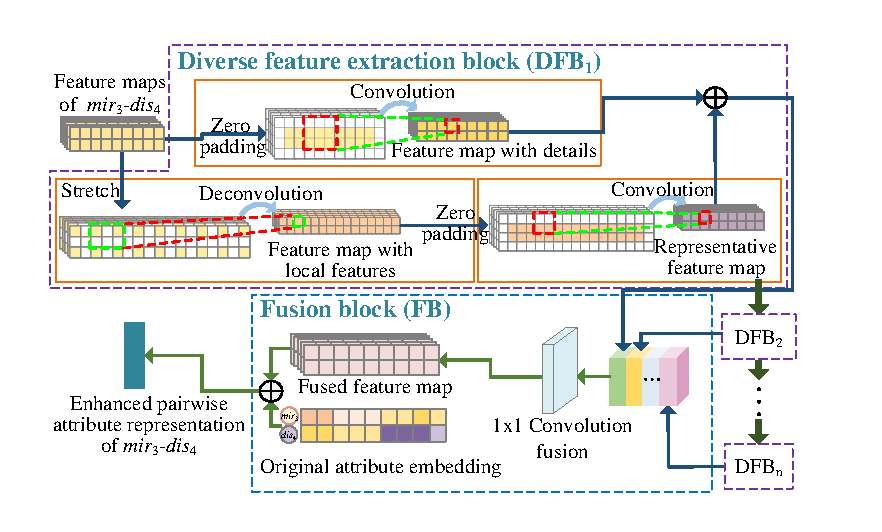
\includegraphics[width=3.5in]{fig/fig-3.pdf}\\
	\caption{ Learning the local feature enhanced attribute representation for a pair of miRNA and disease nodes.}
	\label{fig:03}
	\vspace{-0.4cm}
\end{figure}
%2.5
\subsection{Integrating semantic representation and network-view representation}

The meta-path semantic representation ${Z^{MP}}$ was obtained from the level of semantics implied by each meta-path. A node representation-level attention mechanism was proposed to obtain feature fusion representation with node attention enhancement since ${Z^{MP}}$ and network-view representations ${Z^{Net}}$ have varied contributions to miRNA-disease association prediction. We use the miRNA node $mi{r_i}$ as an example to explain this attention mechanism, with the meta-path semantic representation and network-view representation of $mi{r_i}$ as ${Z^{MP}}\left( i \right)$ and ${Z^{Net}}\left( i \right)$, respectively. 
The following formulas are used to determine the attention score ${w_{i,v}}$ and the accompanying normalized attention weights ${\beta _{i,v}}$.
\begin{equation}
{w_{i,v}} = {a_m}\sigma \left( {W_m^{nft} \cdot \left( {{Z^v}\left( i \right)} \right) + b_m^{nft}} \right),
\end{equation}
\begin{equation}
{\beta _{i,v}} = \frac{{\exp \left( {{w_{i,v}}} \right)}}{{\sum\nolimits_{t \in \left\{ {MP,Net} \right\}} {\exp \left( {{w_{i,t}}} \right)} }},
\end{equation}
where $v \in \left\{ {MP,Net} \right\}$, ${a_m}$ and $W_m^{nft}$ are the weight vector and weight matrix, respectively, $b_m^{nft}$ represents bias vector, and $\sigma $ is the activation function $tanh$. 

The node feature fusion representation of $mi{r_i}$ is denoted as ${T^{nft}}\left( i \right)$.
\begin{equation}
{T^{nft}}\left( i \right) = \sum\nolimits_{v \in \left\{ {MP,Net} \right\}} {\left( {{w_{i,v}}\cdot\left( {{Z^v}\left( i \right)} \right) + {Z^v}\left( i \right)} \right)},
\end{equation}
${T^{nft}}\left( {{N_m} + j} \right)$ is the node feature fusion representation of disease $di{s_j}$.

${T^{nft}}\left( i \right)$ and ${T^{nft}}\left( {{N_m} + j} \right)$ are stitched together left and right to form $K$. Then we obtained the $mi{r_i} - di{s_j}$ association score ${s^{nft}}$ by feeding $K$ to the fully connected layer and the $softmax$ layer,
\begin{equation}
{s^{nft}} = softmax\left( {{W_{nft}} \cdot K + {b_{nft}}} \right),
\end{equation}
where ${W_{nft}}$ and ${b_{nft}}$ denote weight matrix and bias vector of the fully connected layer.

\begin{figure*}
	\centering
	% requires \usepackage{graphicx}
	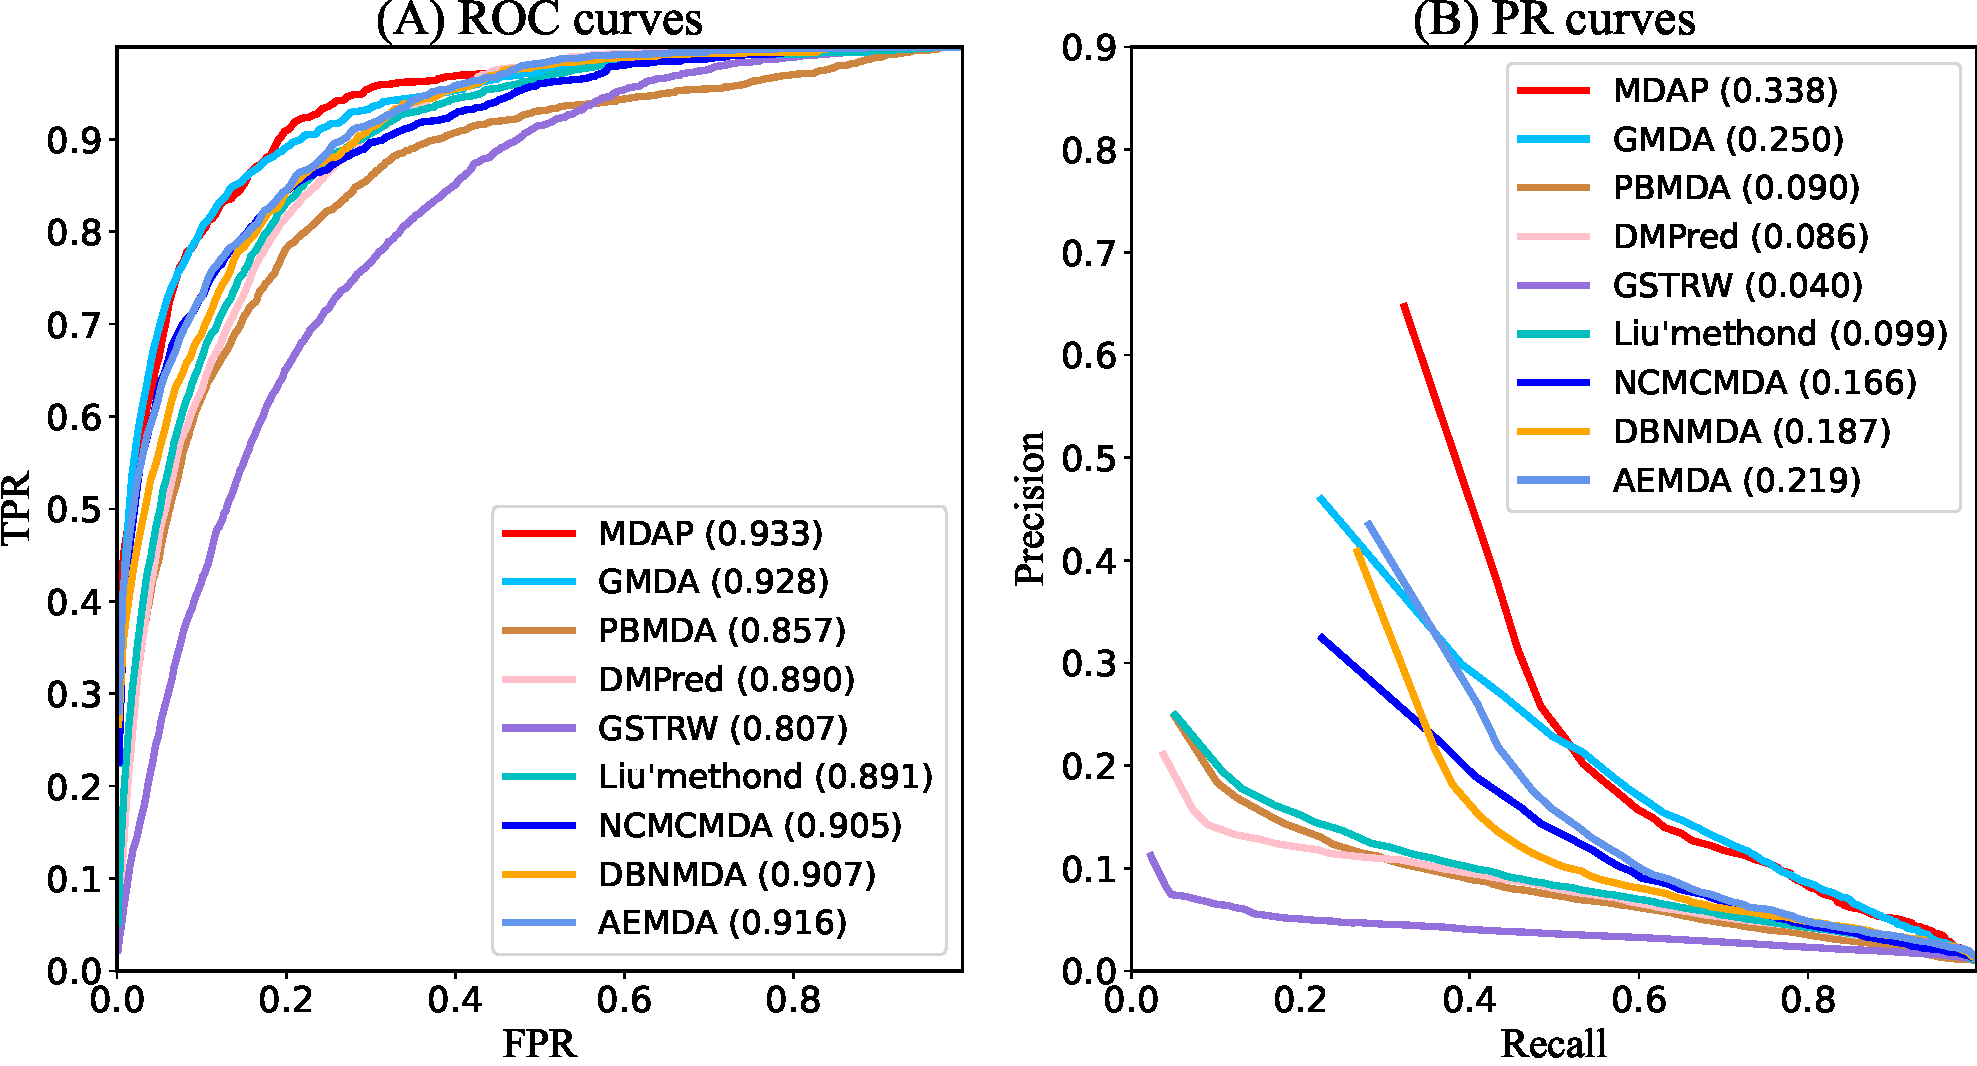
\includegraphics[width=6in]{fig/AUC_AUPR.pdf}\\
	\caption{MDAP and other methods for the area under ROC and PR curves of all diseases.}
	\label{fig:04}
	\vspace{-0.4cm}
\end{figure*}

%2.6
\subsection{Learning of detail and diversity feature enhanced node pair attribute representations}

The feature vectors ${X_i}$ and ${X_{{N_m} + j}}$ of miRNA $mi{r_i}$ and disease $di{s_j}$ were spliced up and down to obtain the paired attribute embedding $H \in {R^{2 \times {N_v}}}$ of $mi{r_i} - di{s_j}$. A parallel convolutional-deconvolutional network was built to extract diverse pairwise node attributes. As shown in Figure \ref{fig:01}(d), the parallel convolution-deconvolution module includes a shallow feature extraction block (SFB), multiple diversity feature extraction blocks (DFB), and a fusion block (FB).  

The SFB consists of a convolutional layer, $H$ is fed into SFB to form the feature map $T_{deh}^s \in {R^{2 \times {N_v}}}$,
\begin{equation}
T_{deh}^s = \delta \left( {W_{deh}^s * H + b_{deh}^s} \right),\end{equation}
where $\delta $ is the activation function $Relu$, weight matrix and bias vector are represented by $W_{deh}^s$ and $b_{deh}^s$, and ' $ * $ ' denotes the convolution operation.

We connected the ${N_{deh}}$ DFBs in series, and the input of each DFB was the output of the previous feature extraction block. Each DFB contains two parallel-connected blocks: a convolution block and deconvolution block. The attribute features of the node pair at the original level are extracted using a convolutional block, which consists of one convolutional layer, and $T_{deh}^s$ is the input to the first convolutional block. To learn the edge information of $T_{deh}^s$, it was filled with 0. 

$T_{deh}^s$ passes through the convolutional layer in the $\psi $ th convolutional block to form the convolutional feature map $T_{deh}^{c,\psi }$,

\begin{equation}
T_{deh}^{c,\psi } = W_{deh}^{c,\psi } * T_{deh}^{c,\psi  - 1} + b_{deh}^{c,\psi },{\rm{ 1}} \le \psi  \le {N_{deh}},
\end{equation}
where ` $ * $ ' represents the convolution operation. $W_{deh}^{c,\psi }$ represents the weight matrix.

One deconvolution layer and a convolution layer constitute the deconvolution block. The deconvolution layer performs an inter-element complementary 0 to the original feature map, stretching its size and making the perceptual field more focused on the local information of the original input. Therefore, this deconvolution layer can learn representative features at the local level in the feature map.

The input of the first deconvolution block is $T_{deh}^s$, which passes through the deconvolution layer of the $\psi $ th deconvolution block to obtain the feature map $T_{deh}^{dc,\psi }$,
\begin{equation}
T_{deh}^{dc,\psi } = W_{deh}^{dc,\psi } \mathrel{\setbox0=\hbox{$\times$}
\rlap{\hbox to\wd0{\hss$\div$\hss}}\box0} T_{deh}^{dc,\psi  - 1} + b_{deh}^{dc,\psi },{\rm{1}} \le \psi  \le {N_{deh}},
\end{equation}
where ` $\divideontimes $ ' denotes the deconvolution operation. $W_{deh}^{dc,\psi }$ and $b_{deh}^{dc,\psi }$ are the weight matrix and the bias vector, respectively, and $T_{deh}^{dc,0} = T_{deh}^s$. 

$T_{deh}^{dc,\psi }$ is then passed through a convolution layer so that it is reprojected to the same dimension as $T_{deh}^{c,\psi }$ to form a deconvolution feature map $T_{deh}^{d,\psi }$,
\begin{equation}
T_{deh}^{d,\psi } = W_{deh}^{d,\psi } * {\rm{ }}T_{deh}^{dc,\psi } + b_{deh}^{d,\psi }{\rm{ ,1}} \le \psi  \le {N_{deh}},
\end{equation}
where ` $ * $ ' represents the convolution operation, $W_{deh}^{d,\psi }$ represents the weight matrix, and $b_{deh}^{d,\psi }$ is the bias vector. 
Thus, after the convolution blocks and deconvolution blocks, we learn the diversity features of the node pairs from different levels. 

In each DFB, we sum the obtained convolution and deconvolution feature maps before feeding the activation function, and then obtain the $\psi $ th diverse feature map $T_{deh}^{M,\psi }$,

\begin{equation}
T_{deh}^{M,\psi } = g\left( {T_{deh}^{c,\psi } + T_{deh}^{d,\psi }} \right),
\end{equation}
where $g$ is the activation function $Relu$. To integrate detailed and diverse node pair features, we established cross-layer connections between individual feature extraction blocks. 

We fused $T_{deh}^{M,1},T_{deh}^{M,2},...,T_{deh}^{M,{N_{deh}}}$ at FB using a 1×1 convolution kernel to obtain the fused diversity feature map $\hat T_{deh}^R$,
\begin{equation}
\hat T_{deh}^R = W_{deh}^R \cdot \left| {T_{deh}^{M,1},T_{deh}^{M,2},...,T_{deh}^{M,{N_{deh}}}} \right| + b_{deh}^R,
\end{equation}
where $\left|  \cdot  \right|$ is the connection operation, $W_{deh}^R$ and $b_{deh}^R$ are weight matrix and bias vector, respectively. Finally, the original feature map was supplemented to retain more original detail information, resulting in detailed and diverse feature-enhanced pairwise attribute representations.

We fed $T_{deh}^R$ into the fully connected layer and $softmax$ layer to calculate the association prediction score ${s^{deh}}$,
\begin{equation}
{s^{deh}} = softmax\left( {{W_{deh}} \cdot T_{deh}^R + {b_{deh}}} \right),\end{equation}
where ${W_{deh}}$ and ${b_{deh}}$ represent the weight matrix and the bias vector, respectively.
%2.7
\subsection{Association prediction score and optimization}

When learning the node feature fusion representation, cross-entropy is applied as a loss function between the association prediction score ${s^{nft}}$ and the real label $t$, defined as
\begin{equation}
Los{s_{nft}} =  - \sum\limits_{i = 1}^{{{{N}}_{tra}}} {\sum\limits_{j = 1}^c {{t_j}\log \left( {{s^{nft}},j} \right)} },
\end{equation}
where ${N_{tra}}$ denotes the number of training sample sets. When there is a real association between $mi{r_i}$ and $di{s_j}$, ${t_j} = 1$; otherwise, ${t_j} = 0$

In the learning process of node pair attribute representation with enhanced detail and diversity features, the cross-entropy loss is $Los{s_{deh}}$,
\begin{equation}
Los{s_{deh}} =  - \sum\limits_{i = 1}^{{{{N}}_{tra}}} {\sum\limits_{j = 1}^c {{t_j}\log \left( {{s^{deh}},j} \right)} },
\end{equation}
We use Adam algorithm \cite{2014Adam} to optimize the loss functions $Los{s_{nft}}$ and $Los{s_{deh}}$, respectively. 

Finally, ${s^{nft}}$ and ${s^{deh}}$ are weighted and integrated to obtain the final predicted score $S$,
\begin{equation}
S = \lambda  \times {s^{nft}} + \left( {1 - \lambda } \right) \times {s^{deh}},
\end{equation}
where $\lambda $ is utilized to modify the contributions of the enhanced node pair attribute information and the node feature fusion representation.

\section{Experimental Evaluations and Discussions}

\subsection{Experimental setup}

In this model, we learn the semantic information of meta-path $miRNA - miRNA$, $miRNA - disease$, $miRNA - miRNA - miRNA$, $disease - disease$, $disease - miRNA$, and $disease - disease - disease$. The dimension of the feature mapping was 600 and the number of neighbor nodes was 50 in the meta-path-encoding module. The network-view representation learning module had 2 encoding layers and 2 decoding layers, and output feature dimensions of 900 and 600 for the encoding layer and 900 and 1134 for the decoding layer. The number of DFB in the parallel convolutional deconvolutional network was two. For each DFB, the deconvolution layer in the deconvolution block had 32 filters of size 2 × 3, 32 filters of size 2 × 2 made up the convolution layer. The convolutional layer in the SFB and the convolutional block of the DFB both had a filter of size 3 × 3. The learning rate was set as 0.0005.

%3.2
\subsection{Evaluation metrics}

The performance of the MDAP and other models used to infer miRNA-associated diseases was assessed using five-fold cross validation. All miRNA-disease associations we know were employed as positive samples, of which 4/5 were used for training and the remaining for testing. Negative samples consisted of all unobserved miRNA-disease associations. Randomly chosen negative samples were added to the training set in an amount equal to the number of positive samples used for training, and the remaining negative samples were used for testing. We used the area under the receiver operating characteristic (ROC) curve (AUC) \cite{0Integration,hajian2013receiver} and the area under the precision-recall (PR) curve (AUPR) as evaluation metrics \cite{saito2015precision}. Prior to obtaining the average of the five outcomes, we first determined the average AUC and AUPR for each fold. Also, biologists typically choose the candidates with the highest rankings for validation. Therefore, we calculate the recall rates for the top-ranked candidates with the highest prediction results and used it as one of the evaluation metrics. 

\subsection{Ablation experiments}

To confirm the contribution of meta-path semantic learning, network-view feature learning, node pair attribute learning, representation-level attention mechanism, and semantic-level attention mechanism to predict miRNA-disease associations, we ran ablation experiments. As shown in Table \ref{tab:01}, the final model MDAP achieved the best performance. Without using the meta-path encoding module to learn meta-path semantic information, the AUC decreased by 1.2 \%, and the AUPR was 4.4\% lower than that of the final model. Without using the GCA to learn heterogeneous network information, the AUC and AUPR were 0.8\% and 7\% lower than those of the final model. Compared to the model without learning node-to-attribute representations, the final model enhanced performance in AUC and AUPR by 1.4\% and 5.8\%. Compared to MDAP, the model without the representation-level attention mechanism showed a decrease of 0.4\% and 2.9\% in AUC and AUPR, respectively, while the model without the semantic-level attention mechanism displayed a 0.3\% and 2.3\% decrease in AUC and AUPR, respectively. The main reason is that representation-level attention and semantic-level attention assign higher weights to more informative node representations and semantic features, which helps to capture the more important features of nodes and improve the prediction performance. The learning of node-pair attributes contributes the most to the improvement in prediction performance, probably because it integrates more local and representative features of the node pairs.

\begin{figure}
	\centering
	%\usepackage{float}
	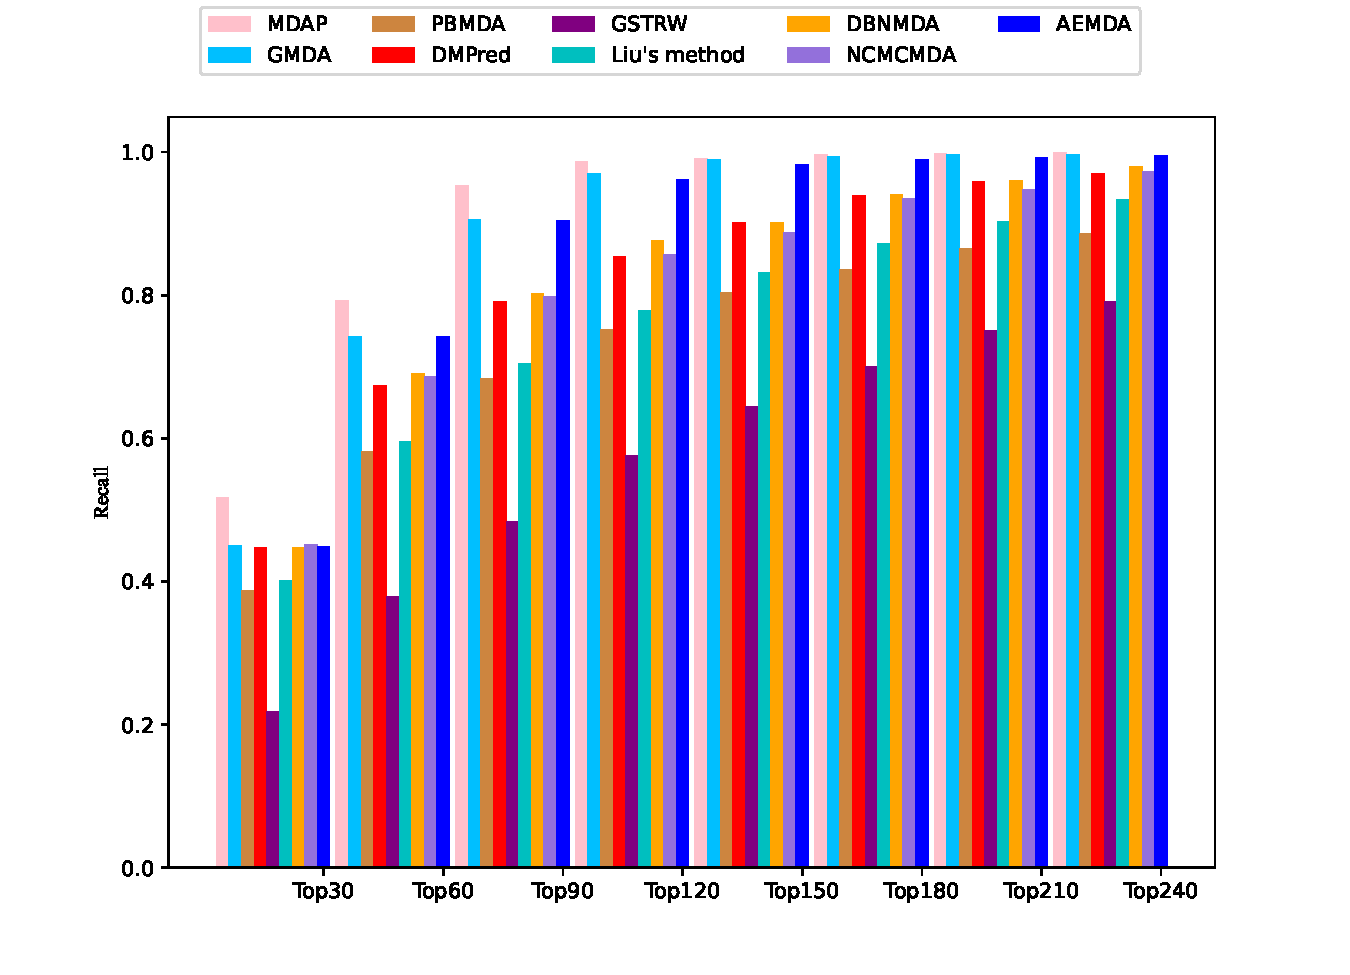
\includegraphics[width=3.5in]{fig/top_k.pdf}\\
	\caption{The recall values at different top $k$ cutoffs.}
	\label{fig:05}
	\vspace{-0.4cm}
\end{figure}


% \begin{table}[!b]
	
% 	\centering	
%     \caption{Results of ablation experiments in our method. }\label{tab:tab1}
%     \label{tab:01}
% 		\begin{tabular}{p{0.9cm}<{\centering} p{0.9cm}<{\centering} p{0.9cm}<{\centering} p{1cm}<{\centering} p{1cm}<{\centering} | p{0.7cm}<{\centering} p{0.7cm}<{\centering}}
% 			\hline
% 			 meta-path semantic learning & network-view feature learning & node pair attribute learning &  representation-level attention & semantic-level attention & Average AUC & Average AUPR \\
% 			\hline
% 		    \ding{55} & \checkmark & \checkmark & \ding{55} & \ding{55} & 0.921 & 0.294 \\
% 		    \checkmark & \ding{55} & \checkmark & \ding{55} & \checkmark & 0.925 & 0.268 \\
% 		    \checkmark & \checkmark & \ding{55} & \checkmark & \checkmark & 0.919 & 0.280\\
%             \checkmark & \checkmark & \checkmark & \ding{55} & \checkmark & 0.929 & 0.309\\
%             \checkmark & \checkmark & \checkmark & \checkmark & \ding{55} & 0.930 & 0.315\\
% 		    \checkmark & \checkmark & \checkmark &  \checkmark & \checkmark & \textbf{0.933}& \textbf{0.338} \\
% 			\hline
% 		\end{tabular}
% \end{table}

\begin{table*}
	\centering
	\begin{threeparttable}[b]
		 \caption{Results of ablation experiments in our method. }\label{tab:tab1}
    \label{tab:01}
		\begin{tabular}{p{2.5cm}<{\centering} p{2cm}<{\centering} p{2cm}<{\centering} p{2cm}<{\centering} p{2cm}<{\centering} | p{1.5cm}<{\centering} p{1.5cm}<{\centering}}
			\hline
			 meta-path semantic learning & network-view feature learning & node pair attribute learning &  representation-level attention & semantic-level attention & Average AUC & Average AUPR \\
			\hline
		    \ding{55} & \checkmark & \checkmark & \ding{55} & \ding{55} & 0.921 & 0.294 \\
		    \checkmark & \ding{55} & \checkmark & \ding{55} & \checkmark & 0.925 & 0.268 \\
		    \checkmark & \checkmark & \ding{55} & \checkmark & \checkmark & 0.919 & 0.280\\
            \checkmark & \checkmark & \checkmark & \ding{55} & \checkmark & 0.929 & 0.309\\
            \checkmark & \checkmark & \checkmark & \checkmark & \ding{55} & 0.930 & 0.315\\
		    \checkmark & \checkmark & \checkmark &  \checkmark & \checkmark & \textbf{0.933}& \textbf{0.338} \\
			\hline
		\end{tabular}
	\end{threeparttable}
\end{table*}
\begin{table*}[!t]
	\centering
	\begin{threeparttable}[b]
		\caption{Results of the paired Wilcoxon test for comparing MDAP and all the other methods. }\label{tab:tab3}
  	     \label{tab:02}
		\begin{tabular}{p{2cm}<{\centering}| p{1.3cm}<{\centering} p{1.3cm}<{\centering} p{1.8cm}<{\centering} p{1.3cm}<{\centering} p{1.3cm}<{\centering} p{1.3cm}<{\centering} p{1.3cm}<{\centering} p{1.3cm}<{\centering}}
			\hline
			 & GMDA & AEMDA & Liu’s Method & PBMDA & DMPred & DBNMDA & GSTRW & NCMCMDA\\
			\hline
			$p$-value of AUC & 7.7079e-15 & 3.2298e-10 & 6.8469e-18	& 7.7299e-29 & 1.1402e-22 & 2.2369e-23 & 6.0409e-17 &5.6358e-30\\
			$p$-value of AUPR & 2.5338e-06	& 7.6841e-05 & 5.8481e-11 & 2.7385e-20 & 1.3601e-16 & 1.5846e-13	& 7.3301e-10 & 4.6582e-21\\
			\hline
		\end{tabular}
	\end{threeparttable}
\end{table*}


\subsection{Comparison with Other Methods}
MDAP was compared with GMDA \cite{0Integration}, AEMDA \cite{0AEMDA}, DBNMDA \cite{34}, NCMCMDA \cite{2020NCMCMDA}, GSTRW \cite{2018Global}, DMPred \cite{20}, PBMDA \cite{2017PBMDA}, and Liu’s method \cite{2016Inferring}. By utilizing the best parameter values available for each method, the best performance of MDAP and the other eight methods was presented. Figure \ref{fig:04} displays the ROC and PR curves for the eight approaches for 341 diseases. For the average AUC across all diseases, MDAP yielded the highest AUC of 0.933, which outperformed GMDA by 0.5\%, was 4.2\% better than Liu's method, was superior to PBMDA by 7.6\%, was 4.3\% and 2.6\% higher than the values of DMPred and DBNMDA, exceeded NCMCMDA by 2.5\%, AEMDA by 1.7\%, and outperformed the worst performing GSTRW by 12.6 \%. Similarly, MDAP obtained the best AUPR value (AUPR = 0.338), which was 8.8\%, 24.8\%, 15.1\%, 23.9\%, 29.8\%, 17.2\%, 11.9\%, and 25.2\% higher than GMDA, PBMDA, DBNMDA, Liu's method, GSTRW, NCMCMDA, AEMDA and DMPred, respectively.

In summary, the proposed MDAP model achieves the best performance, with GMDA and AEMDA in the second and third places, respectively. GMDA is based on generative adversarial networks that integrate the neighboring topology of node pairs. AEMDA uses a deep auto-coding model to learn the potential associations. Both ignore the rich semantic information in meta-paths. DBNMDA is based on a deep belief network that deeply integrates the complex relationships between miRNAs and diseases, but does not consider the details of node-pair attributes and edge information. NCMCMDA is a matrix completion-based model that fully utilizes similarity information. The AUC and AUPR values of Liu’s method are similar to those of DMPred, both of which were modeled based on the random walk and non-negative matrix factorization, respectively. The AUPR of PBMDA was a trifle higher than that of DMPred, yet its AUC was 3.3\% lower than that of DMPred. GSTRW performed much worse than MDAP, mainly because it only considered the similarity relationship between the disease and miRNA and did not consider the association information. The improvement of MDAP over other methods is mainly because of its in-depth learning of more local and representative features of node-pair attributes and the integration of node features at the network and meta-path levels.

We obtained mean five-fold AUC and AUPR results for 341 diseases for each prediction approach. A paired Wilcoxon test was performed using 341 pairwise results when the two methods were compared. The study outcomes are presented in Table \ref{tab:02}. MDAP showed better performance in both AUC and AUPR, with a p-value of 0.05. Figure \ref{fig:05} displays the recall rates for various top $k$ values. More positive samples were obtained when the recall rate was higher. Our model outperformed other methods for different values of k because of the comprehensive learning of the semantic information of nodes for multiple meta-paths, miRNA-disease network information, and property details of node pairs.

MDAP obtained the highest recall rates when k was 30, 60, 90, and 120, with 51.8\%, 79.3\%, 95.3\%, and 98.7\%, respectively. The GMDA and AEMDA also achieved acceptable recall rates. The former had recall rates of 45\%, 74.2\%, 90.6\%, and 97\%, while the latter had 44.9\%, 74.25, 90.4\%, and 96.1\%. When k in the range of 30–120, the values of NCMCMDA were 45.2\%, 68.7\%, 79.8\%, and 85.7\%, respectively. The recall rates for DBNMDA and DMPred were very close, with 44.8\%, 69.1\%, 80.2\%, and 87.6\% for the former and 44.7\%, 67.4\%, 79.1\%, and 85.4\% for the latter corresponding to the rates. When k=30, Liu’s method ranked 40.2\%, and PBMDA ranked 38.8\%. When k ranged from 60 to 120, Liu’s method achieved recall rates of 59.5\%, 70.5\%, and 77.9\%, respectively, and PBMDA obtained rates of 58.1\%, 68.3\%, and 75.2\%. The rates of DSTRW were consistently lower than those of the other methods when the k values ranged from 30 to 120, with rates of 21.8\%, 37.9\%, 48.4\%, and 57.6\%.


\begin{table*}[tb]
	\centering
		\begin{threeparttable}[b]	
		\caption{The top 50 miRNA candidates related to ovarian  neoplasms.}
		\setlength{\tabcolsep}{0mm}	
         \label{tab:03}
		\begin{tabular}{p{1.5cm}<{\centering} p{2.5cm}<{\raggedright} p{4.5cm}<{\raggedright} | p{1.5cm}<{\centering}   p{2.5cm}<{\raggedright} p{4.5cm}<{\raggedright}}
            \hline
            Rank &  MiRNA name & Description & Rank & MiRNA name & Description\\
			\hline
            1 &	hsa-mir-150 & miRCancer, dbDEMC & 26	 & hsa-mir-708 & dbDEMC\\
            2 &	hsa-mir-92a & miRCancer, dbDEMC & 27	 & hsa-mir-499a & dbDEMC\\
            3 & hsa-mir-155 & miRCancer, dbDEMC, miR2Disease & 28 & hsa-mir-381 & dbDEMC, miR2Disease\\
            4 & hsa-mir-34c & miRCancer, dbDEMC, miR2Disease & 29 & hsa-mir-338 & dbDEMC\\
            5 &	hsa-mir-26a & miRCancer, dbDEMC & 30	 & hsa-mir-383 & miRCancer, dbDEMC\\
            6 &	hsa-mir-222 & miRCancer, dbDEMC & 31	 & hsa-mir-302c	 & dbDEMC\\
            7 &	hsa-let-7i & miRCancer, dbDEMC, miR2Disease & 32 & hsa-mir-330 & miRCancer, dbDEMC\\
            8 &	hsa-mir-27a & miRCancer, dbDEMC & 33	 & hsa-mir-363 & miRCancer, dbDEMC\\
            9 &	hsa-mir-194 & miRCancer, dbDEMC & 34	 & hsa-mir-663 & miRCancer, dbDEMC, miR2Disease\\
            10 & hsa-mir-9 & miRCancer, dbDEMC & 35	 & hsa-mir-151	 & dbDEMC\\
            11 & hsa-mir-130a &	miRCancer, dbDEMC & 36	 & hsa-mir-485	 & dbDEMC\\
            12 & hsa-let-7f & dbDEMC, miR2Disease & 37 & hsa-mir-532	 & miRCancer, dbDEMC\\
            13 & hsa-mir-18a & miRCancer, dbDEMC	& 38 & hsa-mir-517a	 & dbDEMC\\
            14 & hsa-mir-10b & dbDEMC, miR2Disease & 39	 & hsa-mir-502	 & dbDEMC\\
            15 & hsa-mir-27b & miRCancer, dbDEMC & 40 & hsa-mir-1202	 & dbDEMC\\
            16 & hsa-mir-429 & miRCancer, dbDEMC, miR2Disease & 41 & hsa-mir-374b & miRCancer, dbDEMC\\
            17 & hsa-mir-101 & miRCancer, dbDEMC & 42 & hsa-mir-1207	 & dbDEMC\\
            18 & hsa-mir-96 & miRCancer, dbDEMC & 43	 & hsa-mir-376c	 & dbDEMC\\
            19 & hsa-mir-98 & miRCancer, dbDEMC & 44	 & hsa-mir-886	 & dbDEMC\\
            20 & hsa-mir-139 & miRCancer, dbDEMC & 45 & hsa-mir-634	 & dbDEMC\\
            21 & hsa-mir-128 & dbDEMC & 46 & hsa-mir-933 & dbDEMC\\
            22 & hsa-mir-497 & miRCancer, dbDEMC & 47 & hsa-mir-519a	& miRCancer, dbDEMC, miR2Disease\\
            23 & hsa-mir-135b & dbDEMC & 48 & hsa-mir-203b & dbDEMC\\
            24 & hsa-mir-320a &	dbDEMC & 49 & hsa-mir-3 & unconfirmed\\
            25 & hsa-mir-370 & dbDEMC & 50 & hsa-mir-15a & miRCancer, dbDEMC\\
			\hline
		\end{tabular}
	\end{threeparttable}
\end{table*}

\subsection{Case studies on 3 diseases}
To further demonstrate the capability of MDAP to identify potential miRNA-disease associations, we conducted case studies on three diseases, including ovarian neoplasms, lung neoplasms, and breast neoplasms. Using ovarian neoplasms as an example, we obtained the association score of its candidate miRNAs through the model and ranked it in decreasing order. For validation and analysis, the top 50 putative miRNAs for ovarian neoplasms were identified. Supplementary Tables ST1 and ST2 list the top 50 potential miRNAs associated with breast and lung neoplasms, respectively.

The miRCancer database contains 9080 experimentally validated miRNA-disease associations, which were extracted from published literature using text mining techniques by Xie {\it et al.} \cite{2013miRCancer} and further verified manually. miR2Disease is a database covering 349 miRNAs, 163 diseases, and 3273 miRNA-disease-related information. As indicated in Table \ref{tab:03}, 27 candidate miRNAs for ovarian neoplasms were identified in miRCancer, and 9 candidate miRNAs were included in miR2Disease. This suggests that the expression of these miRNAs is upregulated or downregulated in ovarian neoplasms.

The integrated database dbDEMC stores differentially expressed miRNAs in cancer, as detected using high-throughput and low-throughput methods \cite{DBLP:journals/nar/YangWWTZZT17}. The database includes 2224 miRNAs and 36 cancers. In our model, 49 of the 50 miRNA candidates associated with ovarian neoplasms were supported by dbDEMC, implying that they were aberrantly expressed in ovarian neoplasm cells. Among the 50 candidates, 1 candidate miRNA was not confirmed by the observed evidence; hence, it was labeled as “unconfirmed”. Supplementary Table ST1 shows 50 candidate miRNAs for breast neoplasms. miRCancer and miR2Disease contain 34 and 13 candidate miRNAs, respectively, suggesting that these miRNAs may be involved in the development of breast neoplasms. Among the 50 candidate miRNAs for lung neoplasms (Supplementary Table ST2), miRCancer included 40 candidate miRNAs. There were 48 candidates recorded by dbDEMC and 15 candidates by miR2Disease, indicating that these miRNAs were indeed associated with lung neoplasms. All case studies show that MDAP is indeed able to discover potential miRNA-disease associations. 

\subsection{Investigation of novel disease-related miRNAs prediction}
We utilized MDAP to infer disease-associated miRNA candidates for 341 diseases. In Supplementary Table ST3, the top 50 miRNA candidates for every disease predicted by MDAP are listed.

\section{Conclusions}
We proposed a miRNA-disease association prediction method, MDAP, for encoding and fusing the semantics from diverse meta-paths and the topological structure and attributes from the entire miRNA-disease network. The constructed multiple meta-paths for the miRNA (disease) nodes are helpful for capturing the high-order neighbor topologies about these meta-paths to learn the semantic features of the miRNA (disease) nodes. A meta-path-sensitive graph convolution module was built for each meta-path and we integrated the various semantic features of the miRNA and disease nodes from multiple meta-paths. A graph convolutional autoencoder was constructed to capture the topological structure and the node attributes from the entire miRNA-disease heterogeneous network. The designed strategy based on parallel convolutional-deconvolutional networks is beneficial for the more local and representative features of each miRNA-disease pair. Two attention mechanisms were proposed to assign greater weights for the more informative meta-paths and node representations. Five-fold cross-validation results showed that MDAP achieved higher AUC and AUPR than the compared methods. MDAP also obtained the more actual disease-related miRNAs in the top-ranked prediction candidates. MDAP’s ability in discovering the potential miRNA-disease associations was illustrated through the case studies on 3 diseases which includes ovarian neoplasms, lung neoplasms, and breast neoplasms.
\bibliographystyle{IEEEtran}
\bibliography{cas-refs}
\end{document}
